\chapter{结果、讨论与展望}
% \chapter{Results, Discussion, and Outlook}
\label{chap:results}

本章在前文信号提取（第\ref{chap:signal-efficiency}章）、效率修正（第\ref{chap:signal-efficiency}章）和系统误差评估（第\ref{chap:systematics}章）的基础上，汇总$pp \to J/\psi + J/\psi + \phi + X$过程的最终物理结果。第\ref{sec:final-candidates-fit}节报告候选事例统计量与拟合结果，第\ref{sec:corrected-results-interp}节给出效率修正后的信号产额与截面测量值，第\ref{sec:comparison-related}节讨论与相关理论和实验工作的联系，第\ref{sec:conclusion-outlook}节总结本分析并给出后续展望。

\section{候选事例与拟合结果}
% \section{Candidate Events and Fit Results}
\label{sec:final-candidates-fit}

按照第\ref{chap:reconstruction-selection}章的选择流程，从$\SI{13.6}{\tera\eV}$质子--质子碰撞数据的$\mu^+\mu^-\mu^+\mu^-K^+K^-$末态中获得$4.8829\times10^4$个$J/\psi J/\psi \phi$候选事例。采用第\ref{chap:signal-efficiency}章所述的三维无分箱扩展最大似然拟合提取信号，三个共振均为真实信号的分量产额为$N_{sss}=(1.563\pm0.143)\times10^3\,(\mathrm{stat})$，信号统计显著性由似然比检验确认为$12.0\sigma$。


\section{修正后结果与物理解释}
% \section{Corrected Results and Physical Interpretation}
\label{sec:corrected-results-interp}

\subsection{效率修正后的信号产额}

利用第\ref{chap:signal-efficiency}章描述的接受度与效率修正框架，基于\DPSone 基准效率图，对每个选定事例赋予修正权重$w = 1/(A_{\mathrm{tot}} \cdot \epsilon_{\mathrm{tot}})$并乘以sWeight信号权重，得到效率修正后的总信号产额：
\begin{equation}
\label{eq:result-corrected-yield}
N_{sss}^{\mathrm{corr}}
=
(9.35 \pm 1.94\,(\mathrm{stat}) \pm 1.76\,(\mathrm{syst,\,partial}))
\times10^4
\end{equation}
其中统计误差由产额修正后不变质量谱拟合不确定度给出。标记为$\mathrm{syst,\,partial}$的第二项仅表示当前已经定量评定的部分系统误差，其数值为18.8\%，来自采用不同子过程MC样本构造效率图时修正后产额的变化（详见第\ref{chap:systematics}章第\ref{subsec:syst-model-dependence}节）。图~\ref{fig:yield-comparison}比较了五种效率情景下的修正后信号产额。排除\SPSLO 情景后，其余四种情景给出的产额范围为$[5.8 \times 10^4, 9.35 \times 10^4]$；以该范围相对于\DPSone 基准值的包络半宽定义当前传播的系统误差分量。


\begin{figure}[htbp]
  \centering
  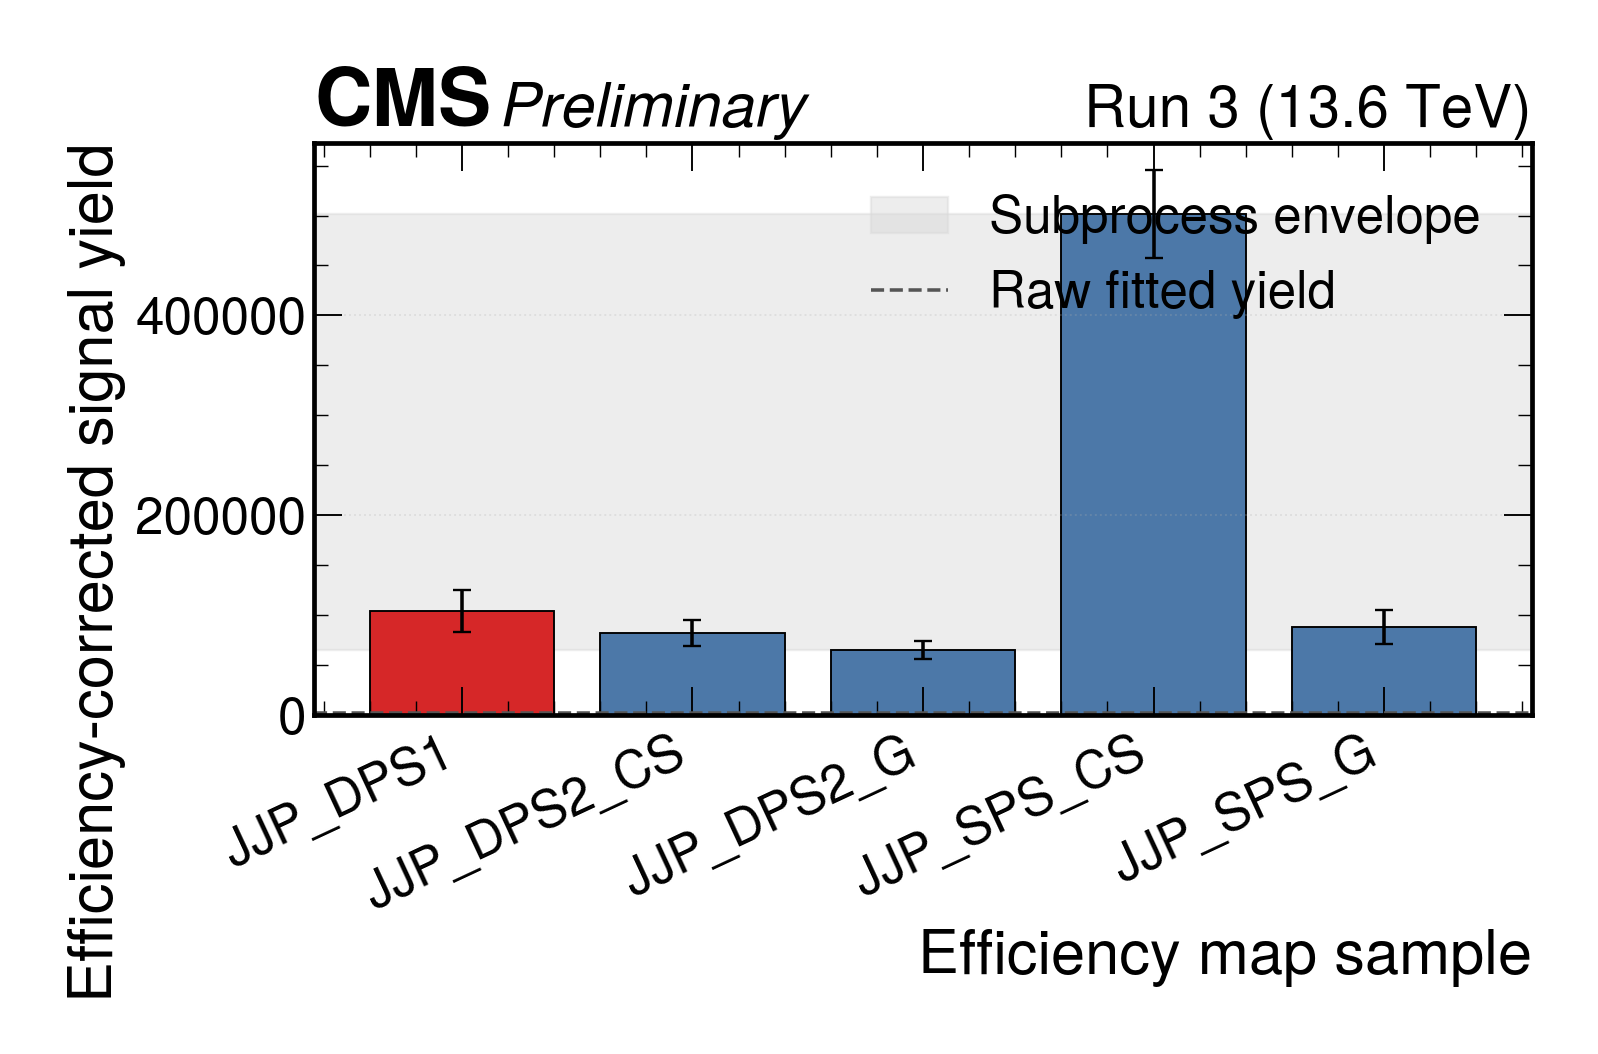
\includegraphics[width=0.65\textwidth]{figures/chap07-results/yield_comparison.png}
  \caption{五种效率变动情景下的修正后$J/\psi J/\psi \phi$信号产额比较。基准结果为\DPSone（红色），误差棒表示统计误差。\SPSLO 情景（内部campaign名为\texttt{JJP\_SPS\_CS}）给出的产额远大于其余四种情景，因其运动学分布对应较低的缪子重建效率，从而放大修正权重。该情景的SPS截面理论预期极低，故不计入标称系统误差包络。}
  \label{fig:yield-comparison}
\end{figure}

\subsection{截面测量}

效率修正后的信号产额与产生截面之间的关系为
\begin{equation}
\label{eq:xsec-relation}
\sigma(pp \to J/\psi + J/\psi + \phi + X) \times \mathcal{B}^2(J/\psi \to \mu^+\mu^-) \times \mathcal{B}(\phi \to K^+K^-) = \frac{N_{sss}^{\mathrm{corr}}}{\mathcal{L}_{\mathrm{int}}},
\end{equation}
其中$\mathcal{L}_{\mathrm{int}} = \SI{289.21 \pm 5.97}{\per\femto\barn}$为积分亮度（第\ref{chap:experiment-dataset}章）。代入数值得到
\begin{equation}
\label{eq:result-xsec-times-BR}
\sigma \times \mathcal{B}^2(J/\psi \to \mu^+\mu^-) \times \mathcal{B}(\phi \to K^+K^-) = 323 \pm 67\,(\mathrm{stat}) \pm 61\,(\mathrm{syst,\,partial})~\SI{}{\femto\barn}
\end{equation}

利用世界平均分支比$\mathcal{B}(J/\psi \to \mu^+\mu^-) = (5.961 \pm 0.033)\%$和$\mathcal{B}(\phi \to K^+K^-) = (49.9 \pm 0.5)\%$~\cite{PDG2024}，进一步得到绝对产生截面：
\begin{equation}
\label{eq:result-xsec}
\sigma(pp \to J/\psi + J/\psi + \phi + X) = 182 \pm 38\,(\mathrm{stat}) \pm 34\,(\mathrm{syst,\,partial})~\SI{}{\pico\barn}
\end{equation}

式~\eqref{eq:result-xsec-times-BR}和式~\eqref{eq:result-xsec}中的$\mathrm{syst,\,partial}$与式~\eqref{eq:result-corrected-yield}采用相同定义，仅传播不同子过程MC效率图所给出的18.8\%变化。该标签不代表完整的实验系统误差。

\subsection{物理解释}

测量得到的$\SI{182 \pm 38}{\pico\barn}\,(\mathrm{stat}) \pm \SI{34}{\pico\barn}\,(\mathrm{syst,\,partial})$截面显著大于典型SPS产生多夸克偶素末态的微扰QCD预期。对于包含两个$J/\psi$候选和一个$\phi$候选的末态，单次硬散射需要同时产生双粲偶素系统，并通过伴随部分子辐射和强子化形成$\phi$候选，因而受到高阶耦合和多重强子形成概率的压低。相比之下，DPS机制可将不同介子分配到相互独立的硬散射中，有望给出更大的产生率。本分析测得的较大截面支持MPS贡献占优的产生图景，与双$J/\psi$产生中DPS贡献占优的实验证据一致~\cite{CMS_TRI_JPSI}。不同子过程MC效率图之间的比较（第\ref{chap:systematics}章第\ref{subsec:syst-model-dependence}节）表明，采用\SPSLO 样本得到的效率图会给出远大于其他情景的修正产额（$\sim 2.5 \times 10^5$），反映出该样本运动学与数据之间存在明显差异。

\section{与相关工作的比较}
% \section{Comparison with Related Work}
\label{sec:comparison-related}

$J/\psi J/\psi \phi$的伴随产生是本分析首次在实验上进行探索的末态。此前，CMS合作组已在$\sqrt{s} = \SI{13}{\tera\eV}$下观测到了三重$J/\psi$产生~\cite{CMS_TRI_JPSI}以及$Y(1S)$对产生~\cite{CMSY1SY1S13TeV2020}；ATLAS和LHCb合作组也在不同能量下测量了双$J/\psi$产生截面~\cite{ATLAS_JPSIJPSI_8TEV,LHCbJpsiJpsi13TeV2017,LHCbJpsiJpsi13TeV2024}。然而，在有意义地比较不同末态的绝对截面之前，需要计算有效截面（$\sigma_{\mathrm{eff}}$）以扣除部分子分布函数的依赖，从而将不同的多重夸克偶素过程置于同一标度下讨论。有效截面的提取需要额外的理论输入和实验测量，目前尚未完成，因此本节暂不进行定量的过程间比较。

\section{结论与展望}
% \section{Conclusion and Outlook}
\label{sec:conclusion-outlook}

本文围绕 CMS 实验中 \(pp \to J/\psi + J/\psi + \phi + X\) 联合产生过程，
完成了候选事例选择、三维质量谱信号提取、接受度与效率修正、系统误差评估框架以及截面结果讨论的论文整理。
本分析在$\sqrt{s}=\SI{13.6}{\tera\eV}$质子--质子碰撞数据中重建
\(\mu^+\mu^-\mu^+\mu^-K^+K^-\)末态，
并通过三维无分箱扩展最大似然拟合提取三个共振均为真实信号的成分。
基于当前效率修正和已评定的系统误差分量，测得的截面量级显著高于典型SPS预期，
因而支持该末态中多重部分子散射贡献占优的物理图景。

本分析同时受到若干尚待完善因素的限制。
当前结果中标记为$\mathrm{syst,\,partial}$的误差仅包含采用不同子过程MC样本构造效率图时得到的18.8\%变化，
不能解释为完整的实验系统误差，也不能据此判断其为所有系统误差源中的主导项。
信号与本底拟合模型、固定参数和拟合区间、MC统计与效率分箱、
缪子和带电径迹效率、触发与顶点选择、事例堆积、
积分亮度及分支比等误差源仍需完成定量验证和统一传播。
此外，当前结果主要给出总截面量级和定性机制判断，
尚未完成有效截面\(\sigma_{\mathrm{eff}}\)提取以及与双夸克偶素、三重夸克偶素相关过程的统一定量比较。

后续工作应优先完成其余系统误差源的定量评估，
固化最终候选选择与信号提取方案，
并在统一的理论输入下计算\(\sigma_{\mathrm{eff}}\)。
在统计量和模拟样本允许的情况下，
进一步开展\(J/\psi J/\psi \phi\)系统横动量、快度差和方位角关联等微分分布研究，
将有助于区分SPS、DPS和可能的TPS贡献，
并为多重部分子散射和质子内部多部分子关联提供更直接的实验约束。
